
\label{sec:relate}


\begin{figure*}[t]
	\centering
	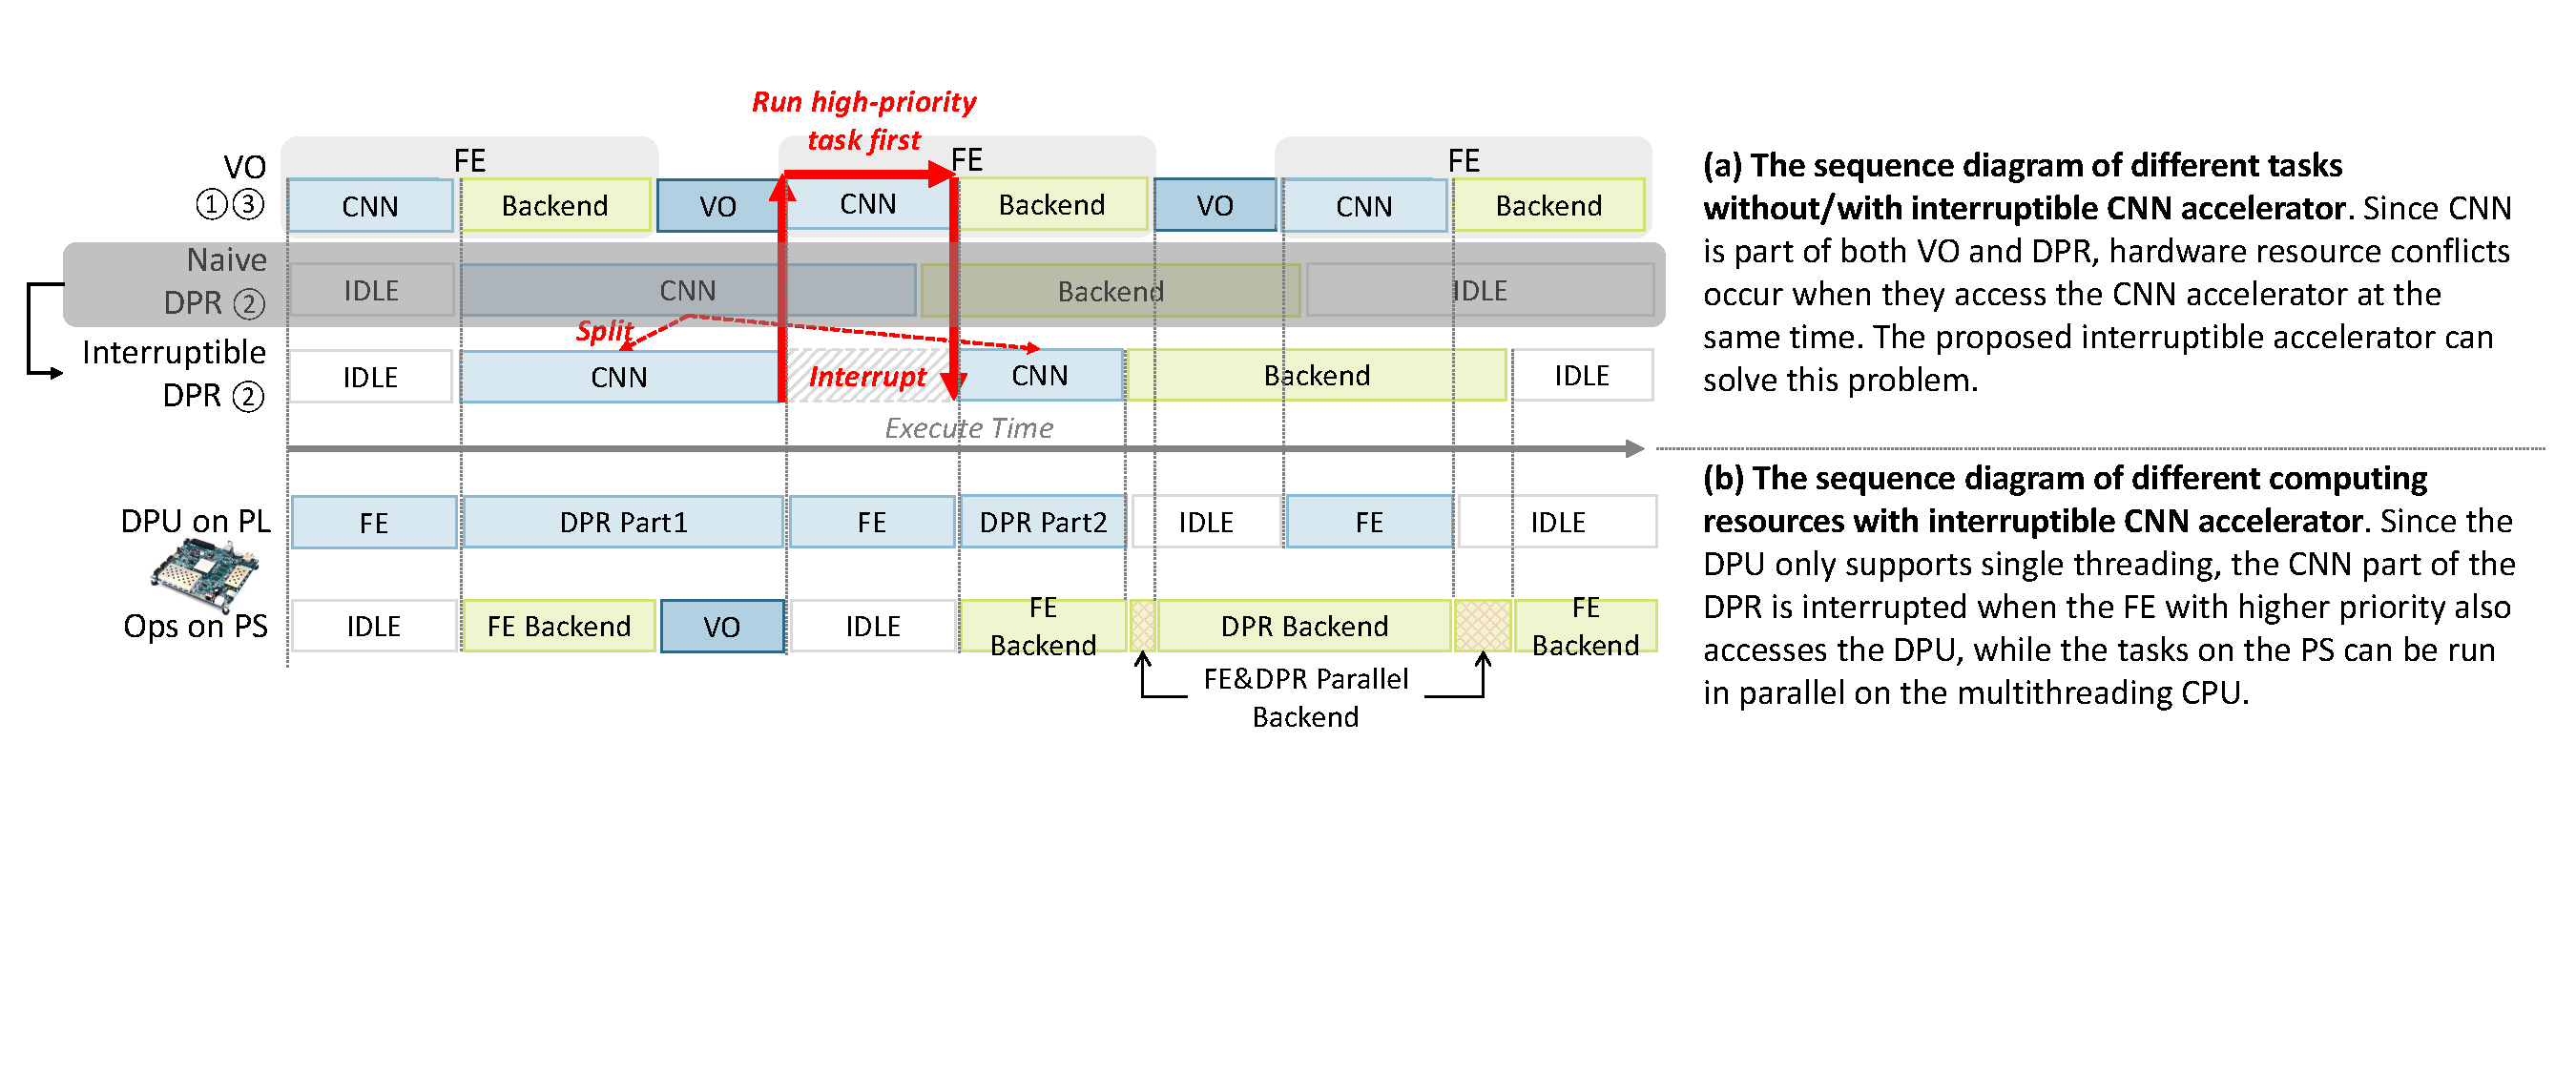
\includegraphics[width=0.99\linewidth]{fig/interDPR.pdf}
    \caption{Interruption to solve the hardware resources conflicts.  
    % When a high-priority task (FE) is started before the low-priority task (PR) is completed, the CNN accelerator backs up the status of PR to memory, and processes the FE task. When the high-priority task is completed, the low-priority task resumes and continues.
    }
	\label{fig:interDPR}
\end{figure*}


\subsection{ CNN-based FE and PR }

\textbf{\quad \ Feature-point extraction:} Previous feature-point extraction works usually consist of two parts: 1) feature-point detection and 2) descriptors generation.
Mur-Artal \cite{Mur-Artal:2017281} proposes a popular open-source SLAM system, ORB-SLAM. ORB-SLAM uses the oFAST (OrientedFeature from Accelerated Segment Test \cite{biadgie2014feature}) detector to locate the feature-points and the BRIEF (Binary Robust Independent ElementaryFeatures \cite{calonder2010brief}) to generate the descriptor for each feature-point in binary strings. 
Simo-Serra \cite{simo2015discriminative} proposes a CNN-based descriptor generator that does not perform any feature-point detection. 
DeTone \cite{detone2018superpoint} presents a fully CNN-based feature-point extraction method, SuperPoint, that implements feature-point detection and descriptors generation using one CNN network. SuperPoint\cite{detone2018superpoint} reaches 10\%-30\% higher matching accuracy compared the ORB based feature-point extraction \cite{Mur-Artal:2017281} and is used in this work.

\textbf{Place recognition:} Before CNN was introduced into place recognition, BoW \cite{small_1} models relying on handcrafted representation is the most popular method. The accuracy of BoW-based methods is strongly influenced by the size of codebooks. Larger codebooks(~1M) \cite{large_1, large_2} can compete with CNN-based methods in accuracy, but they take up huge storage and communication resources. Smaller codebooks\cite{small_1, small_2} require less space but get worse results. In contrast to traditional methods, CNN-based methods not only perform well but also generate compact features. GeM \cite{radenovic2018fine} outperforms other state-of-art CNN-based place recognition methods like NetVLAD \cite{arandjelovic2016netvlad} and is used in this work.


\subsection{ FPGA accelerators for robotic applications }

The feature-point extraction (FE) operation is the basic element of a visual-based robot.
Some previous works design hardware architectures for FE.
SRI-SURF \cite{jia2016sri} optimizes the memory access to speed up SURF \cite{bay2006surf} feature-point extraction method. 
Fang \cite{fang2017fpga} directly implements ORB on FPGA using HLS. Liu \cite{liu2019eslam} optimizes the ORB algrithm and designs a hardware for better performance.
Some other works design architectures for the entire robot system. Hero \cite{shi2018hero} is a framework for navigation and laser-based SLAM and cannot support visual-based SLAM, which is much more lightweighted and cheaper. These specific architectures only support a narrow field of applications. 
Li \cite{li2019879gops} introduces CNN accelerators in robot hardware architecture, making it possible to support evolution of future algorithms. 
However, the CNN accelerator in this work\cite{li2019879gops} is only used for feature-point extraction, and the accelerator is not to support different tasks at the same time.



\subsection{ Scheduling mode of CNN accelerators }

To accelerate CNN on FPGA, some previous works design frameworks to generate a specific hardware architecture for a target CNN, based on  RTL \cite{li_high_2016} or HLS \cite{lu_evaluating_2017}. These works need to reconfigure the FPGA to switch between different CNN models. The reconfiguration comsumes seconds [??], which is unacceptable for the real time system.
Some other works design instruction-driven accelerators \cite{yu2018instruction,qiu2016going,guo2017angel}, making rapid switching possible by providing different instruction sequences. 
However, the CNN tasks on previous instruction-driven CNN accelerators are not interruptible, resulting in the latency-sensitive high-priority task waiting for the low-priority task to finish. This inability of CNN accelerators to support multi-task makes it difficult for robotics researchers to use embedded FPGA.

% However, previous instruction-driven CNN accelerators need to schedule the entire CNN, and can not automatically schedule two or more tasks simultaneously. The inability of CNN accelerators to support multi-task makes it difficult for robotics researchers to use embedded FPGA.